\chapter{Theoretical background}
\label{ch:theoreticalbackground}

\section{What is a system?}
\label{sec:tbsystem}

\textcite[p. 162]{Dietz2020}

A (homogeneous) system can be conceived as a triple ($\mathbb{C}$, $\mathbb{E}$, $\mathbb{S}$), where: \bigskip

\noindent $\mathbb{C}$ is a set of elements, all belonging to the same category,

\indent called the composition of the system;\bigskip

\noindent $\mathbb{E}$ is a set of elements of the same category as the elements in $\mathbb{C}$,

\indent called the environment of the system;\bigskip

\noindent $\mathbb{S}$ is a set of influencing bonds among the elements in $\mathbb{C}$ and between them and the elements in $\mathbb{E}$,

\indent called the structure of the system.


\subsection{Open vs Closed vs Adaptive systems}
\label{sub:tbopenclosedadaptivesystems}
Complex adaptive system (CAS)\\

Quote from AMS011: \parencite{Turner2019}\\
''The whole is different from the sum of its parts and their interactions'' [61] (p.77) Though emergence, the whole cannot be reduced to the original parts, the whole is considered a new entity or unit. The whole is ''qualitatively different from their parts ... The cannot be meaningfully compared-they are different'' [61] (system holism)\\
CAS is going against the second law of thermodynamics.\\

\subsection{Linear and non-linear systems}
\label{sub:linearnonlinear}



\subsection{To be worked upon}

\begin{itemize}
	\item{Senge (systems theory)}
	\item{Cynefone (systems theory)}
	\item{Seneca's Barbbell (Hydra's Body) (Antifragile)}
	\item{Diversity is a thing of reality and needed.}
\end{itemize}

\section{Antifragile}
\label{sec:tbantifragile}

Antifragile loves both randomness and uncertainty.

\begin{itemize}
	\item{Randomness}
	\item{Variability}
	\item{Hormesis / Mithridatisation (by taleb) / Antidotum Mithridatium}
\end{itemize}

It is important to realize that the degree of \gls{fragility} of a system is often a function of its internal structure. The ability of a system to change under stress is governed by the interconnectedness of its parts, how strongly they are tied to each other, and how much change ripples through the system \parencite[p. 886]{OReilly2019}.\\



\subsection{What is a stressor?}
\label{sub:stressor}
As \textcite[p. 54]{Taleb2012} points out ''Stress is knowledge (and knowledge is stress).''

\subsection{Volatile, uncertain, complex, and ambiguous}
\label{seb:tbvuca}

\Gls{volatile}, \gls{uncertain}, \gls{complex}, and \gls{ambiguous}.

\subsection{Relation between antifragile, fragile, robust, resilient, and agile}
\label{sub:tbrelatedtoantifragile}

\gls{antifragile} with \gls{fragile}, \gls{robust}, \gls{resilient}, and \gls{agile}.

\subsection{Resilience}
\label{sub:tbresilience}
\textcite[p. 5-7]{MartinBreen2011} distinguishes three types of resilience:
\begin{itemize}
	\item{\textbf{Engineering Resilience.} Bounce back faster after stress, enduring greater stresses, and being disturbed less by a given amount of stress.}
	\item{\textbf{Systems Resilience.} Maintaining system function in the event of a disturbance. Systems resilience has been applied in governance and management, where it is often called robustness.}
	\item{\textbf{Resilience in Complex Adaptive Systems.} The ability to withstand, recover from, and reorganise in repsonse to crisis. The function is maintained by the system structure may not be. The main differentiator is the adaptive capacity or adaptability of the system.}
\end{itemize}

\begin{figure}[h!]
	\centering
	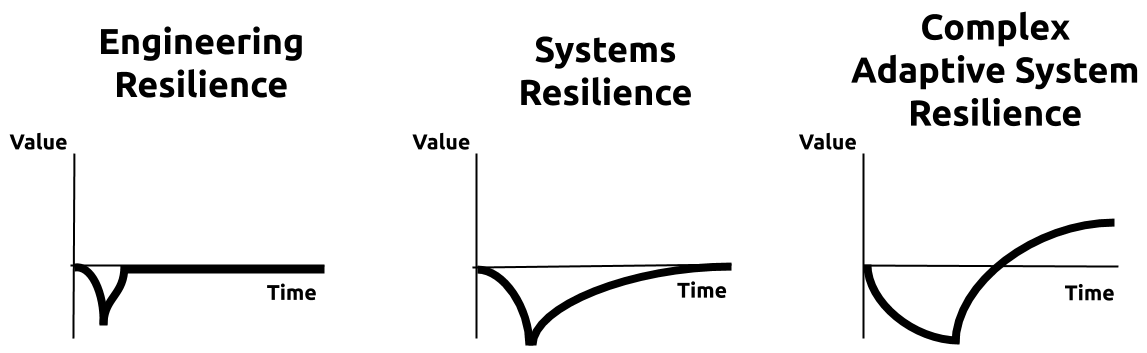
\includegraphics[width=0.7\linewidth]{images/eaal-martin-breen}
	\caption[Three types of resilience]{Three types of resilience \parencite{Botjes2020}}
	\label{fig:eaal-martin-breen}
\end{figure}




\subsection{Antifragile Systems Design}
\label{sub:backgroundasd}



\subsection{Residuality Theory}
\label{sub:residualitytheory}



\section{Enterprise Architecture}
\label{sec:tbea}

\begin{remark}
For example, Ylinen and Pekkola (2018, 2020) recognized two distinct groups of EA experts: a modeling-focused group forming a comprehensive view of an organization and a development-focused group using EA for organizational development. \parencite[p. 16]{Nurmi2021}

Kotusev et al. (2015) reviewed the relevant literature and found three approaches to EA management (EAM): traditional, Massachusetts Institute of Technology (MIT), and dynamic. As discussed by Kotusev et al. (2015), the traditional approach to EAM consists of four phases: documenting the current state, developing the future state, and developing and implementing a transition plan. The MIT approach “advocates the development of a core diagram reflecting a long-term enterprise-level architectural vision.” Finally, the supporting core of the dynamic approach is “just enough, just in time,” meaning no EA is designed until there is a need for it. (Kotusev et al., 2015, p. 4072.)
\end{remark}

There are various understandings of \acrlong{ea} and there is no agreement on them. The various definitions are not always complementary but sometimes in opposite \parencite{Lapalme2012,SaintLouis2019,Hoogervorst2009}.

\textcite{White2018} states that the organisations business requirements guide enterprise architecture — it helps layout how information, business and technology flow together. While \textcite{Gartner} states that Enterprise Architecture is a discipline for proactively and holistically leading enterprise responses to disruptive forces by identifying and analysing the execution of change toward desired business vision and outcomes. EA delivers value by presenting business and IT leaders with signature-ready recommendations for adjusting policies and projects to achieve targeted business outcomes that capitalise on relevant business disruptions. \textcite[p. 9]{Ross2014} defines \acrshort{ea} as the organizing logic for business processes and IT infrastructure, reflecting the integration and standardization requirements of the company’s operating model. The enterprise architecture provides a long-term view of a company’s processes, systems, and technologies so that individual projects can build capabilities—not just fulfill immediate needs. \textcite[p. 24]{Greefhorst2011} defines \acrshort{ea} as those properties of an enterprise that are necessary and sufficient to meet its essential requirements.

\subsection{Three schools of Enterprise Architecture}
\label{sub:eathreeschools}
There are three schools of Enterprise Architecture \parencite{Lapalme2012}:
\begin{itemize}
	\item{\textbf{Enterprise IT Architecting.} Inputs are business strategy and objectives.}
	\item{\textbf{Enterprise Integrating.} It is grounded in systems thinking. It has a holistic view. The link between strategy and execution. Inputs are business strategy and objectives.}
	\item{\textbf{\acrfull{eea}.} Fostering organisational learning by designing all facets of the enterprise, including the relation to its environment.}
\end{itemize}

 \textcite{Lapalme2012} defined the scope of \acrshort{eea} ''the enterprise in its environment, including not only the enterprise but also its environment and the bidirectional relationship and transactions between the enterprise and its environment'' with the purpose to ''help the organization innovate and adapt by designing the various enterprise facets to maximize organizational learning throughout the enterprise.'' As \textcite{Botjes2020} concluded with his \acrshort{eaal} model the attribute learning organisation is of importance for being \gls{resilient} or \gls{antifragile}. If the learning organisation is one of the conditions to be \gls{antifragile} the practice of \acrshort{ea} should be of the school of \acrshort{eea}. 

The properties of an \acrshort{eea} are:

\begin{longtable}{p{.2\textwidth}p{.8\textwidth}}
	\toprule
	& \textbf{\acrlong{eea}} \\ \midrule%
%	\multicolumn{2}{c}{\textbf{\acrlong{eea}}} \\ \midrule%
	\endhead%
	\hline
	\caption{\acrlong{eea}}
	\label{tab:eaeea}	
	\endfoot%
	Motto    		& Enterprise architecture is the means for organizational innovation and sustainability \\
	Objectives and 	& Innovate and adapt    \\
	concerns		& Support organizational coherence \\
					& Encourage system-in-environment coevolution \\
	Principles and  & Apply a holist (systemic) stance \\
	assumptions		& System-in-environment coevolution  \\
					& Environment can be changed \\
					& Jointly design all organisational dimensions \\
	Skills 			& Foster dialogue \\
					& Apply system and system-in-environment thinking \\
	Challenges		& Foster sensemaking \\
					& Encourage systems thinking and systems-in-environment paradigm shifts \\
					& Collaborate across the organisation \\
	Insights		& Fosters system-in-environment coevolution and enterprise choherency \\
					& Fosters organisational innovation and sustainability \\
	Limitation		& Requires many organisational preconditions for management and strategy creation \\
	\bottomrule
\end{longtable}

\subsection{Steering mechanisms}
\label{sub:tbeasteering}

\section{Public sector}
\label{sec:tbpsmarket}
I argue that, in the hybrid model, the definition of the public sector is not correct anymore. The part of a private company that is a part of a hybrid collaboration with the public sector should be part of the definition of the public sector.

\begin{figure}[H]
	\centering
	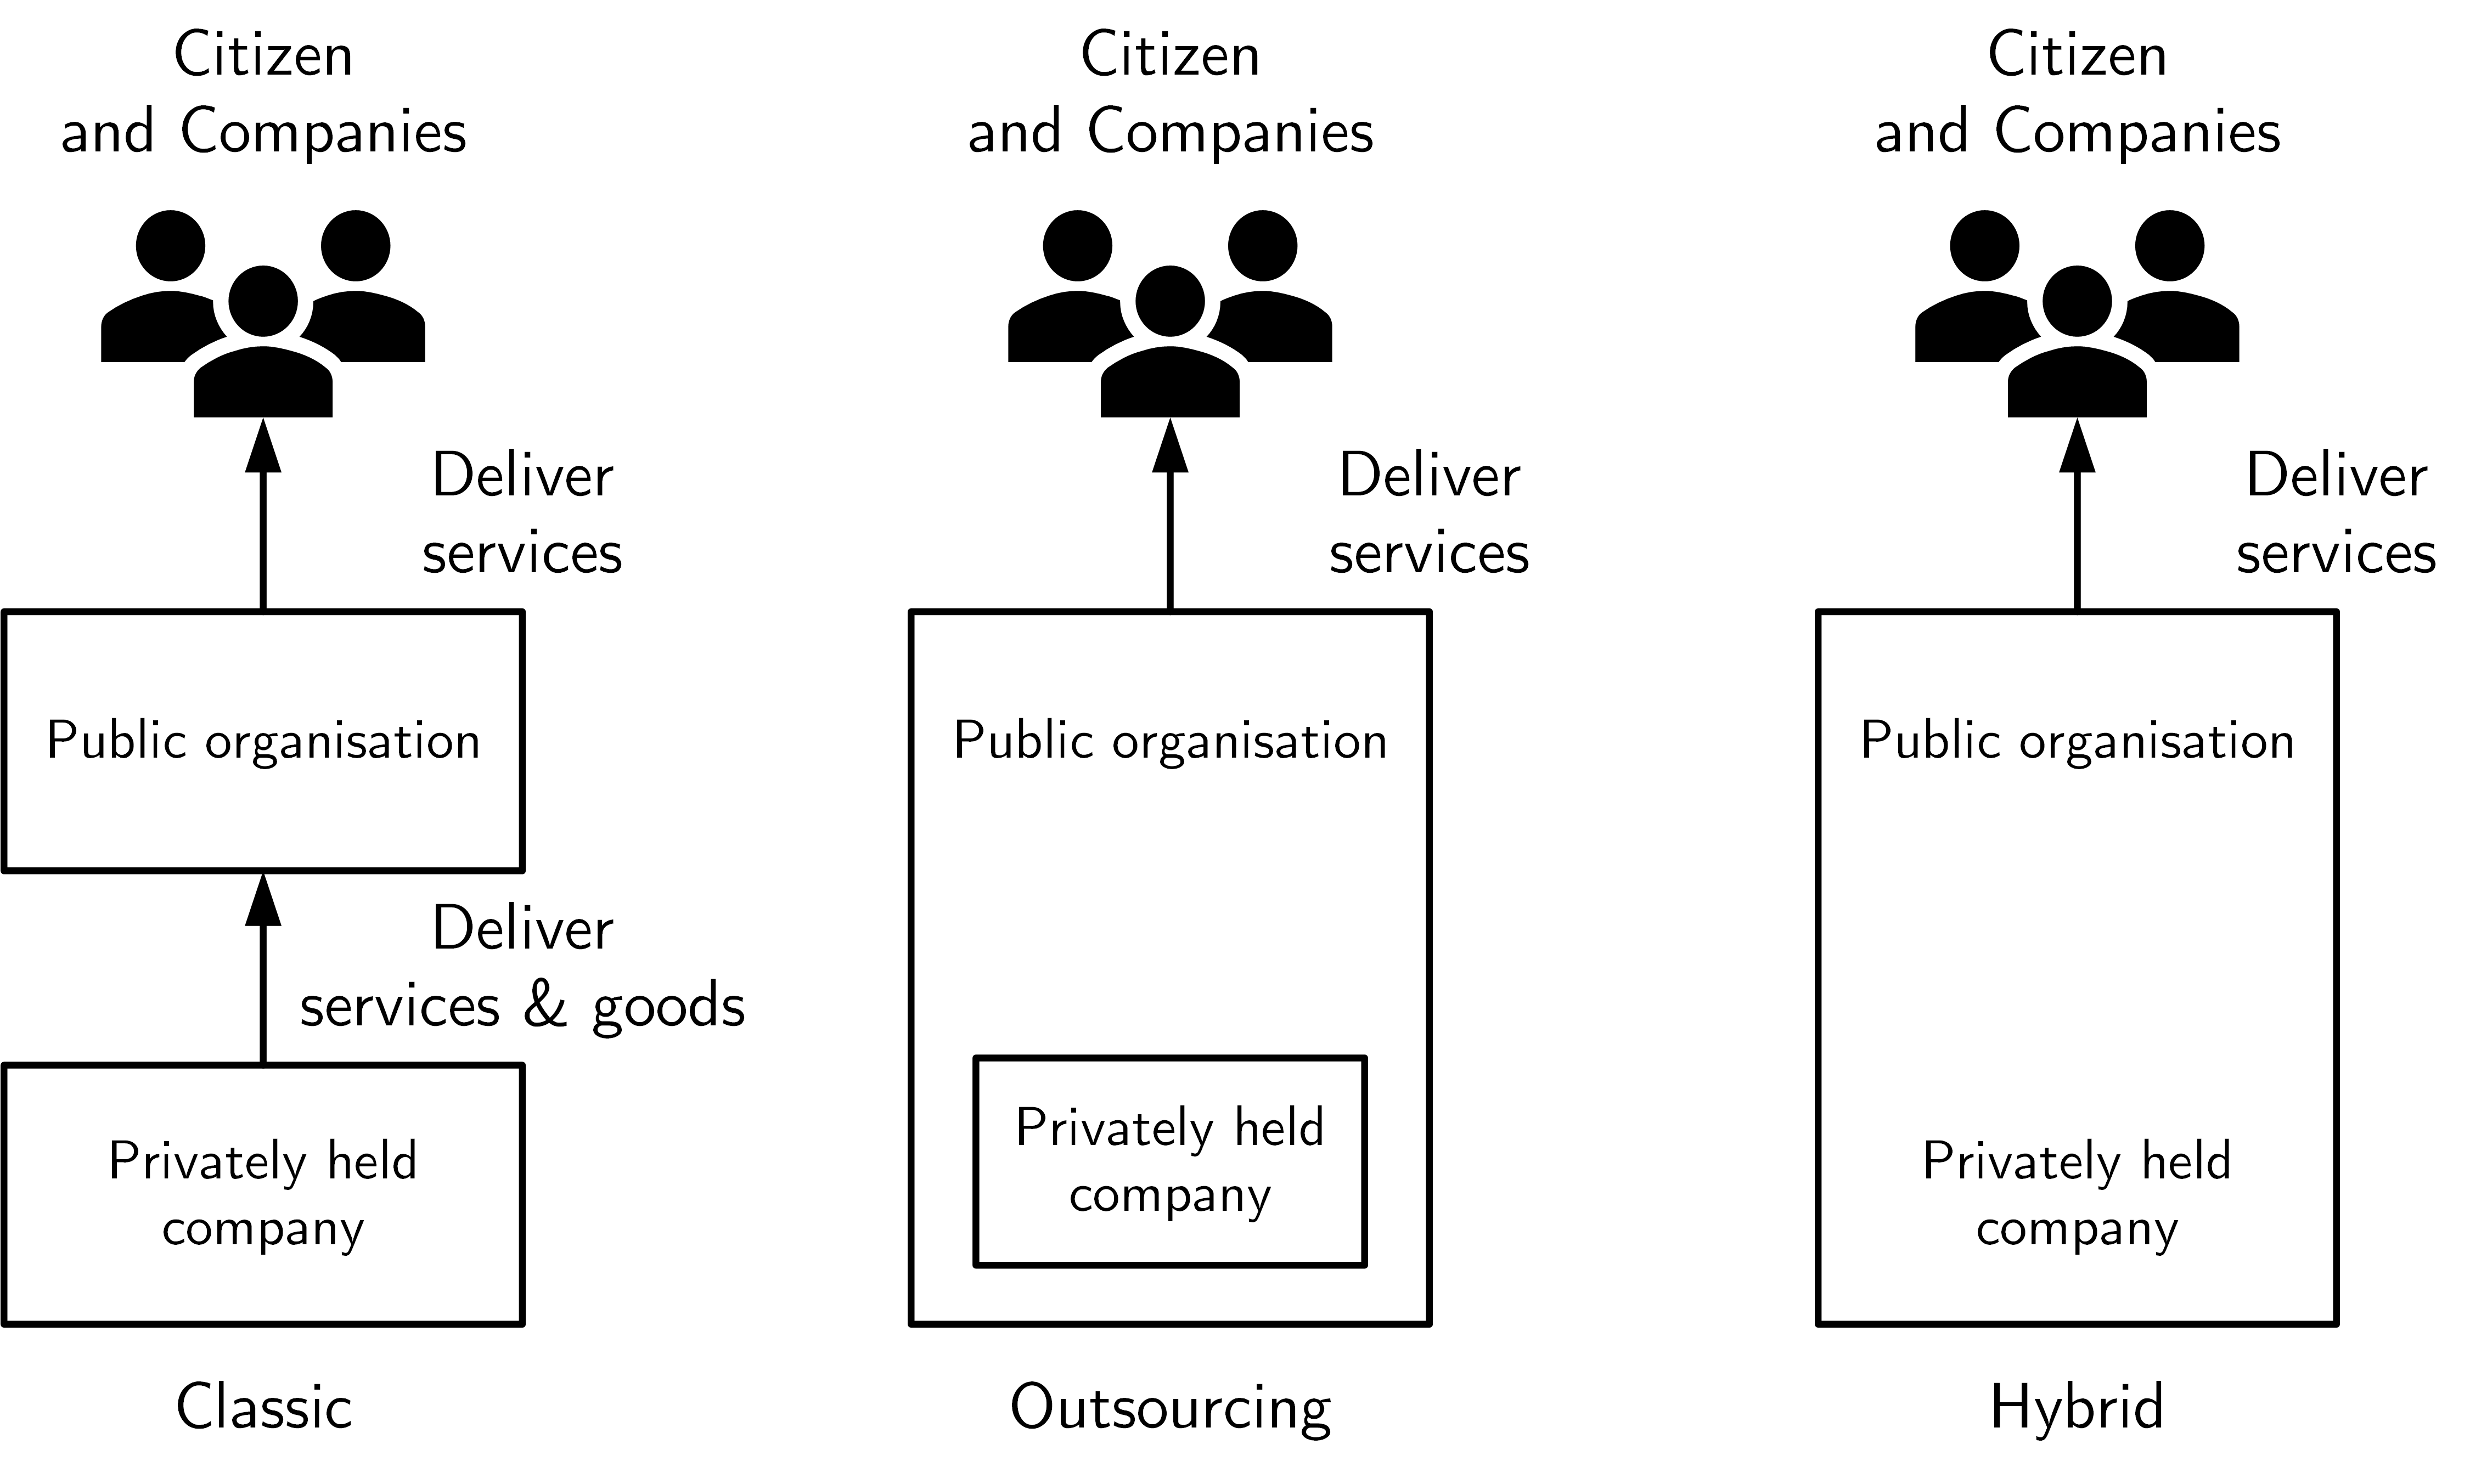
\includegraphics[width=0.7\linewidth]{images/publicsector3modelsofcolaboration}
	\caption[Public sector collaboration models]{Public sector collaboration models}
	\label{fig:publicsector3modelsofcolaboration}
\end{figure}

The public sector is divided into three levels \parencite{PrivacySense2016}:

\begin{itemize}
	\item{\textbf{The national government,} such as the military, the tax authority, and homeland affairs.}
	\item{\textbf{The regional government,} such as the provinces, the police, and water management.}
	\item{\textbf{The local government,} such as the municipalities, the social services, and the local tax offices.}
\end{itemize}

I will focus this research on the public sector level local government of the Netherlands. In \cref{ch:discussion} I will discuss the applicability on non Dutch public sectors.


\begin{remark}
	For hybrid collaborations and partnerships add the reference to iBestuur congress of 2021 about the necessity for the public and private sector to work closely together. Public Sector sees this as necessary to speed up innovation. The reference is expected first week of October 2021.
\end{remark}

\begin{remark}
	The analysis of the 3 types of collaboration should go to the theoretical background. Is necessary to state that the public sector includes privately held companies in some way. Possible even a System-of-Systems.
\end{remark}

\begin{remark}
	Local government is influenced by national government because of policies and regulations.
\end{remark}
\subsection{Differences with the Private Sector Market}
\label{sub:tbdifferenceprivatesector}

The core values are different in the public sector than that of the private sector. The top five private sector core values are profitability, accountability, expertise, reliability, and effectiveness. The top five public sector core values are accountability, effectiveness, incorruptibility, reliability, and lawfulness. \parencite{Wal2008} Profitability is only a value for the private sector, and it does not exist as a value for the public sector.  The public sector demands or even initiates changes without noticing the needed investments to execute these changes by the private sector.
